\subchapter
{New packages in Buildroot}
{Objectives:
  \begin{itemize}
  \item Create a new package for {\em nInvaders}
  \item Understand how to add dependencies
  \item Add patches to {\em nInvaders} for {\em Nunchuk} support
  \end{itemize}
}

\section{Preparation}

After doing a Google search, find the {\em nInvaders} website and
download its source code. Analyze its build system, and conclude which
Buildroot package infrastructure is the most appropriate to create a
package for {\em nInvaders}.

\section{Minimal package}

Create a directory for the package in the Buildroot sources,
\code{package/ninvaders}. Create a \code{Config.in} file with one
option to enable this package, and a minimal \code{ninvaders.mk} file
that specifies what is needed just to {\em download} the package.

For reference, the download URL of the {\em nInvaders} tarball is
\code{http://downloads.sourceforge.net/project/ninvaders/ninvaders/0.1.1/}.

Note: to achieve this, only two variables need to be defined in
\code{.mk} file, plus the call to the appropriate package
infrastructure macro.

Now, go to \code{menuconfig}, enable {\em nInvaders}, and run
\code{make}. You should see the {\em nInvaders} tarball being
downloaded and extracted. Look in \code{output/build/} to see if it
was properly extracted as expected.

\section{Make it build!}

As you have seen in the previous steps, {\em nInvaders} uses a simple
\code{Makefile} for its build process. So you'll have to define the
{\em build commands} variable to trigger the build of {\em
  nInvaders}. To do this, you will have to use four variables provided
by Buildroot:

\begin{itemize}

\item \code{TARGET_MAKE_ENV}, which should be passed in the
  environment when calling \code{make}.

\item \code{MAKE}, which contains the proper name of the \code{make}
  tool with potentially some additional parameters to parallelize the
  build.

\item \code{TARGET_CONFIGURE_OPTS}, which contains the definition of
  many variables often used by \code{Makefiles}: \code{CC},
  \code{CFLAGS}, \code{LDFLAGS}, etc.

\item \code{@D}, which contains the path to the directory where the
  {\em nInvaders} source code was extracted.

\end{itemize}

When doing Buildroot packages, it is often a good idea to look at how
other packages are doing things. Look for example at the \code{jhead}
package, which is going to be fairly similar to our \code{ninvaders}
package.

Once you have written the {\em nInvaders} build step, it's time to
test it. However, if you just run \code{make} to start the Buildroot
build, the \code{ninvaders} package will not be rebuilt, because it
has already been built.

So, let's force Buildroot to rebuild the package by removing its
source directory completely:

\begin{verbatim}
make ninvaders-dirclean
\end{verbatim}

And then starting the build:

\begin{verbatim}
make
\end{verbatim}

This time, you should see the \code{ninvaders 0.1.1 Building} step
actually doing something, but quickly failing with a message saying
that the \code{ncurses.h} file could not be found.

Move on to the next section to see how to solve this problem!

\section{Handling dependencies}

The \code{ncurses.h} header file is missing, because {\em nInvaders}
depends on the \code{ncurses} library for drawing its interface on a
text-based terminal. So we need to add \code{ncurses} in the
dependencies of {\em nInvaders}. To do this, you need to do two
things:

\begin{itemize}

\item Express the dependency in the package \code{Config.in} file. Use
  a \code{select} statement to make sure the \code{ncurses} package
  option is automatically selected when \code{ninvaders} is
  enabled. Check that the \code{ncurses} package does not have itself
  some dependencies that need to be propagated up to the
  \code{ninvaders} package.

\item Express the dependency in the package \code{.mk} file.

\end{itemize}

Restart again the build of the package by using
\code{make ninvaders-dirclean all} (which is the same as doing
\code{make ninvaders-dirclean} followed by \code{make}).

Now the package should build properly! If you look in
\code{output/build/ninvaders-0.1.1/}, you should see a
\code{nInvaders} binary file. Run the \code{file} program with
\code{nInvaders} as argument to verify that it is indeed built for
ARM.

However, while \code{nInvaders} has been successfully compiled, it is
not installed in our target root filesystem!

\section{Installing and testing the program}

If you study the {\em nInvaders} \code{Makefile}, you can see that
there is no provision for installing the program: there is no
\code{install:} rule.

So, in \code{ninvaders.mk}, you will have to create the {\em target
  installation commands}, and simply manually install the
\code{nInvaders} binary. Use the \code{$(INSTALL)} variable for
that. Again, take example on the \code{jhead} package to know how to
achieve that.

Rebuild once again the \code{ninvaders} package. This time, you should
see the \code{nInvaders} binary in \code{output/target/usr/bin/}!

Reflash your root filesystem on the SD card and reboot the
system. {\em nInvaders} will not work very well over the serial port,
so log to your system through \code{ssh}, and play \code{nInvaders}
with the keyboard!

Note: if you get the error \code{Error opening terminal:
  xterm-256color.} when running \code{nInvaders}, issue first the
command \code{export TERM=xterm}.

\section{Support the Nunchuk}

Playing with the keyboard is nice, but playing with our Nunchuk would
be even nicer! We have written a patch for {\em nInvaders} that makes
this possible.

This patch is available in the lab data directory, under the name
\code{0001-joystick-support.patch}. Copy this patch to the right
location so that it gets applied after {\em nInvaders} is extracted by
Buildroot, and before it is built. Rebuild once again the
\code{ninvaders} package. Verify that the patch gets applied at the
\code{ninvaders 0.1.1 Patching} step.

However, this patch relies on the Linux kernel {\em joystick
  interface}, that we need to enable. Go to the Linux kernel
configuration using \code{make linux-menuconfig}, and enable
\code{CONFIG_INPUT_JOYDEV}. Exit, and make sure to save your kernel
configuration safely using \code{make linux-update-defconfig}. Restart
the overall build by running \code{make}.

Then reflash your kernel image and root filesystem on the SD card,
reboot, and start {\em nInvaders} in a SSH session. You should now be
able to control it using the Nunchuk joystick, and fire with the
\code{C} button.

\section{Adding a hash file}

To finalize the package, add the missing {\em hash file}, so that
people building this package can be sure they are building the same
source code. To know the hash, SourceForge provides this information:
go to the {\em nInvaders} download page, and next to the file name,
there is a small information icon that will provide the MD5 and SHA1
hashes. Add both hashes to the hash file.

\begin{center}
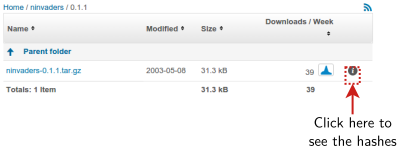
\includegraphics[width=\textwidth]{labs/buildroot-new-packages/hashes-on-sourceforge.pdf}
\end{center}

Once the {\em hash file} is added, rebuild the package completely by
doing \code{make ninvaders-dirclean all}.

Look at the build output, and before the \code{ninvaders 0.1.1
  Extracting} step, you should see a message like this:

\begin{verbatim}
ninvaders-0.1.1.tar.gz: OK (sha1: ....)
ninvaders-0.1.1.tar.gz: OK (md5: ....)
\end{verbatim}

\section{Testing package removal}

Now, to experiment with Buildroot, do the following test: disable the
\code{ninvaders} package in \code{menuconfig} and restart the build
doing \code{make}. Once the build is done (which should be very
quick), looked in \code{output/target/}. Is {\em nInvaders} still
installed? If so, why?
